\documentclass[10pt,xcolor=dvipsnames]{beamer}
\usepackage[french]{babel}
\usepackage[utf8]{inputenc}
\usepackage[T1]{fontenc}
\usepackage{caption}
\usepackage{MnSymbol,wasysym}
\usepackage{amsmath}
\usepackage{cancel}
\usepackage[draft]{pdfcomment}
\newcommand{\pdfnote}[1]{\marginnote{\pdfcomment[icon=note]{#1}}}
\usepackage{appendixnumberbeamer}
\usepackage{comment}

\usepackage{pifont}% http://ctan.org/pkg/pifont
\newcommand{\cmark}{\textbf{\textcolor{darkspringgreen}{\ding{51}}}}%
\newcommand{\xmark}{\textbf{\textcolor{red}{\ding{55}}}}%

\usepackage{pgffor}

\renewcommand{\thefootnote}{\fnsymbol{footnote}}



\newcommand*\Let[2]{\State #1 $\gets$ #2}
\usepackage{algorithm}
\usepackage[noend]{algpseudocode}
\usepackage{tcolorbox}

\newtcolorbox{mybox}[3][]
{
  colframe = #2!25,
  colback  = #2!10,
  coltitle = #2!20!black,  
  title    = {#3},
  #1,
}

\usetheme[progressbar=frametitle,numbering=fraction]{metropolis}
%LS:
\setbeamercolor{background canvas}{bg=white}  
\usepackage{appendixnumberbeamer}

\usepackage{booktabs}
\usepackage[scale=2]{ccicons}
\usepackage{tikz}
\usetikzlibrary{calc}
\usepackage{color}
\usepackage{mathtools}

\usetikzlibrary{shapes,snakes}
%% Color Definition
\definecolor{darkspringgreen}{rgb}{0.09, 0.45, 0.27}
\definecolor{push}{HTML}{00AF37}
\definecolor{pull}{HTML}{3319BC}

\newcommand{\push}[1]{\textcolor{push}{push(#1)}}
\newcommand{\pull}[1]{\textcolor{pull}{pop(#1)}}
\newcommand{\pop}{\textcolor{pull}{pop()}}

\newcommand{\defin}[1]{\textcolor{darkspringgreen}{#1}}
\setbeamertemplate{frame footer}{Rohan Fossé}

\setbeamercolor{footline}{fg=gray}

\def\checkmark{\tikz\fill[scale=0.4,color=darkspringgreen](0,.35) -- (.25,0) -- (1,.7) -- (.25,.15) -- cycle;}
\usepackage{pgfplots}
\usepgfplotslibrary{dateplot}

\usepackage{eso-pic}
\usepackage{xspace}
\long\def\/*#1*/{}

\title{
Algorithmique et structure de données
}
\subtitle{Structures de données - suite}

\date{\centering 18 Octobre 2021}
\author{\centering \bf Rohan Fossé}


\begin{document}

\maketitle

\section{Rappels}
\begin{frame}{Rappel du cours précédent}

    \begin{alertblock}{Les piles}
    Une \alert{pile} est une liste linéaire d'objets où les consultations, les insertions et les suppressions se font du même côté. On dit que c'est le \alert{dernier arrivé, premier servi}.
    \end{alertblock}
    \only<2->{
    \begin{alertblock}{Les listes}
    Une \alert{liste chaînée} désigne en informatique une structure de données représentant une collection ordonnée et de taille arbitraire d'éléments de même type.
    \end{alertblock}
    }
    \only<3->{
    \begin{alertblock}{Les files}
      La \alert{file} est une structure de données abstraite, un peu similaire aux piles. Contrairement aux piles, une file d'attente est ouverte à ses deux extrémités.
      On dit que c'est le \alert{premier arrivé, premier servi}.
    \end{alertblock}
    }
    \only<4->{
    \begin{alertblock}{Les arbres binaires}
        \alert{L'arbre binaire} a une condition spéciale : chaque nœud peut avoir un maximum de deux enfants.
    \end{alertblock}
    }
\end{frame}

\begin{frame}{Rappel sur les arbres binaire de recherche}
\begin{exampleblock}{Rappel}
     \defin{L'arbre de binaire de recherche} (ou ABR)  présente un comportement particulier. L'enfant gauche d'un nœud doit avoir une valeur inférieure à celle de son parent et l'enfant droit du nœud doit avoir une valeur supérieure à celle de son parent.     
\end{exampleblock}

    
    \begin{figure}
    \centering
    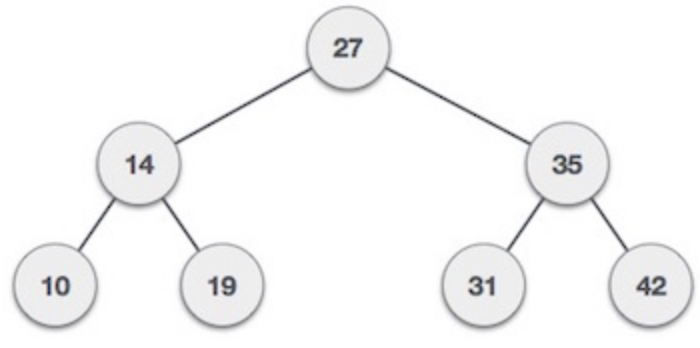
\includegraphics[scale=0.3]{figures/CM2/ABR-2.png}
    \label{fig:my_label}
\end{figure}
    
\end{frame}

\section{AVL}

\begin{frame}{Les AVL}
\only<1>{
    Que se passe-t-il si l'entrée de l'arbre de recherche binaire est triée (ascendante ou descendante) ? Il ressemblera alors à ceci :
}
    \begin{figure}
        \centering
        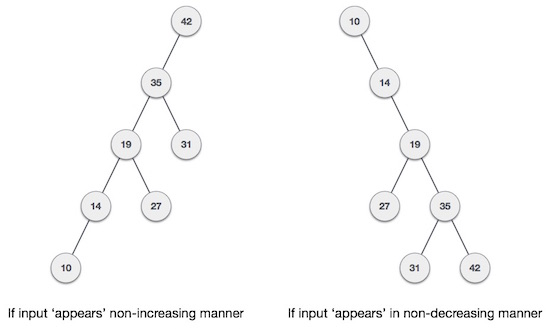
\includegraphics[scale=0.4]{figures/CM3/AVL-unbalanced.jpg}
        \label{fig:my_label}
    \end{figure}
    
\only<2>{

On observe que la performance de recherche dans les \alert{ABR} dans le pire des cas est la plus proche des algorithmes de recherche linéaire, soit $\mathcal{O}(n)$. . Ainsi, on a besoin d'utiliser une méthode pour équilibrer les \alert{ABR}.
}
\end{frame}

\begin{frame}{Les AVL}
\only<1>{
    \begin{exampleblock}{Définition}
        Nommés d'après leur inventeur \textit{Adelson, Velski et Landis}, les arbres \defin{AVL} sont des arbres de recherche binaire à équilibrage de hauteur. L'arbre \defin{AVL} vérifie la hauteur des sous-arbres de gauche et de droite et s'assure que la différence n'est pas supérieure à 1. Cette différence est appelée \defin{\textbf{le facteur d'équilibre}}.
    \end{exampleblock}
    
}
\only<2>{
\begin{figure}
    \centering
    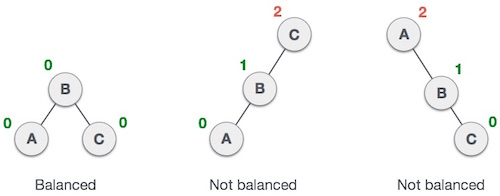
\includegraphics[scale=0.45]{figures/CM3/AVL-balancing.jpg}
    \label{fig:my_label}
\end{figure}
\begin{itemize}
    \item \underline{Deuxième arbre:} le sous-arbre gauche de \textbf{C} a une hauteur de \textbf{2} et le sous-arbre droit a une hauteur de \textbf{0}, la \alert{différence} est donc de \textbf{2};
    \item  \underline{Troisième arbre:} le sous-arbre droit de \textbf{A} a une hauteur de \textbf{2} et le sous-arbre gauche a une hauteur de \textbf{0}, la \alert{différence} est donc de \textbf{2}.
\end{itemize}

}
\only<3>{
    \begin{exampleblock}{Le facteur d'équilibre}
        Facteur-équilibre = taille(sous-arbre-gauche) - taille(sous-arbre-droit)
        
    \end{exampleblock}

    Si la différence de hauteur entre les sous-arbres gauche et droit est supérieure à \textbf{1}, l'arbre est équilibré à l'aide de certaines techniques de rotation.
}
\end{frame}

\begin{frame}{Rotations des AVL}
    Pour s'équilibrer, un arbre \defin{\textbf{AVL}} peut effectuer les quatre types de rotations suivants:


\begin{itemize}
    \item Rotation vers la \alert{gauche};
    \item Rotation vers la \alert{droite};
    \item Rotation \alert{gauche-droite};
    \item Rotation \alert{droite-gauche}.
\end{itemize}
    

Les deux premières rotations sont des rotations simples et les deux suivantes sont des rotations doubles. Pour avoir un arbre déséquilibré, il nous faut au moins un arbre de hauteur \textbf{2}.
\end{frame}

\begin{frame}{Rotation vers la gauche}
    Si un arbre devient déséquilibré, lorsqu'un nœud est inséré dans le sous-arbre droit du sous-arbre droit, nous effectuons alors une seule rotation vers la gauche:
    
    \begin{figure}
        \centering
        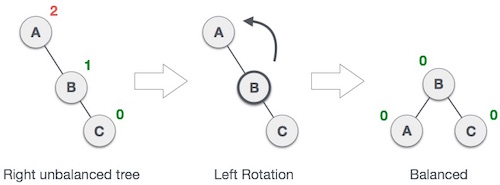
\includegraphics[scale=0.5]{figures/CM3/avl-gauche.jpg}
        \label{fig:my_label}
    \end{figure}
\end{frame}

\begin{frame}{Rotation vers la droite}
    Si un arbre devient déséquilibré, lorsqu'un nœud est inséré dans le sous-arbre gauche du sous-arbre droite, nous effectuons alors une seule rotation vers la gauche:
    
        \begin{figure}
        \centering
        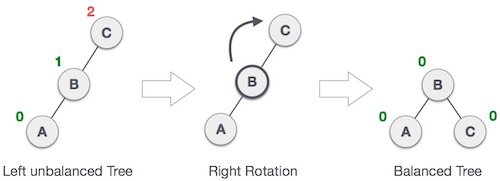
\includegraphics[scale=0.5]{figures/CM3/avl-droit.jpg}
        \label{fig:my_label}
    \end{figure}
\end{frame}


\begin{frame}{Rotation gauche-droite}
\only<1>{
    Les \textbf{doubles rotations} sont une version légèrement plus complexe des versions déjà expliquées des rotations. Voyons d'abord comment effectuer une rotation \alert{gauche-droite}. Une rotation \alert{gauche-droite} est une combinaison d'une rotation \alert{gauche} suivie d'une rotation \alert{droite}.
    }
    
    \only<2>{
    Un nœud a été inséré dans le sous-arbre de droite du sous-arbre de gauche. Cela fait de C un nœud déséquilibré. Ces scénarios font que l'arbre AVL effectue une rotation gauche-droite.
    
    \begin{figure}
        \centering
        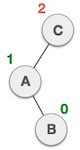
\includegraphics{figures/CM3/avl-gauche-droit-1.jpg}
        \label{fig:my_label}
    \end{figure}
    }
    
    \only<3>{
    Nous effectuons d'abord la rotation gauche sur le sous-arbre gauche de C. Cela fait de A, le sous-arbre gauche de B.
    
    \begin{figure}
        \centering
        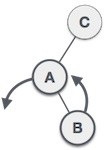
\includegraphics{figures/CM3/avl-gauche-droit-2.jpg}
        \label{fig:my_label}
    \end{figure}
    }
    
    
    \only<4>{
    Le nœud C est toujours déséquilibré, mais maintenant, c'est à cause du sous-arbre gauche du sous-arbre gauche.
    
    \begin{figure}
        \centering
        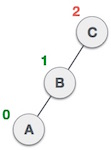
\includegraphics{figures/CM3/avl-gauche-droit-3.jpg}
        \label{fig:my_label}
    \end{figure}
    }
    
    \only<5>{
    Nous allons maintenant effectuer une rotation à droite de l'arbre, faisant de B le nouveau nœud racine de ce sous-arbre. C devient maintenant le sous-arbre droit de son propre sous-arbre gauche.
    
    \begin{figure}
        \centering
        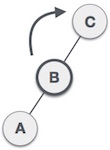
\includegraphics{figures/CM3/avl-gauche-droit-4.jpg}
        \label{fig:my_label}
    \end{figure}
    }
    
    \only<6>{
    L'arbre est maintenant équilibré.
    
    \begin{figure}
        \centering
        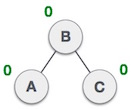
\includegraphics{figures/CM3/avl-gauche-droit-5.jpg}
        \label{fig:my_label}
    \end{figure}
    }
\end{frame}



\begin{frame}{Rotation droite-gauche}

    \only<1>{
    Le deuxième type de double rotation est la rotation droite-gauche. Il s'agit d'une combinaison de la rotation droite suivie de la rotation gauche.
    
    Un nœud a été inséré dans le sous-arbre gauche du sous-arbre droit. Cela fait de A, un nœud déséquilibré avec un facteur d'équilibre de 2.
    
    \begin{figure}
        \centering
        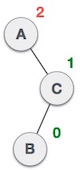
\includegraphics{figures/CM3/avl-droit-gauche-1.jpg}
        \label{fig:my_label}
    \end{figure}
    }
    
    \only<2>{
        Tout d'abord, nous effectuons une rotation vers la droite le long du nœud C, faisant de C le sous-arbre droit de son propre sous-arbre gauche B. Maintenant, B devient le sous-arbre droit de A.
        
        \begin{figure}
            \centering
            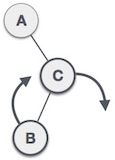
\includegraphics{figures/CM3/avl-droit-gauche-2.jpg}
            \label{fig:my_label}
        \end{figure}
    }
    
    \only<3>{
    Le nœud A est toujours déséquilibré à cause du sous-arbre droit de son sous-arbre droit et nécessite une rotation vers la gauche.
    
    \begin{figure}
        \centering
        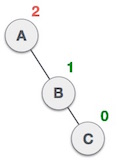
\includegraphics{figures/CM3/avl-droit-gauche-3.jpg}
        \label{fig:my_label}
    \end{figure}
    }
    
    \only<4>{
    Une rotation vers la gauche est effectuée en faisant de B le nouveau nœud racine du sous-arbre. A devient le sous-arbre gauche de son sous-arbre droit B.
    
    \begin{figure}
        \centering
        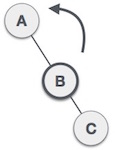
\includegraphics{figures/CM3/avl-droit-gauche-4.jpg}
        \label{fig:my_label}
    \end{figure}
    }
    
    \only<5>{
            L'arbre est maintenant équilibré. 
        \begin{figure}
        \centering
        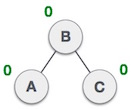
\includegraphics{figures/CM3/avl-droit-gauche-5.jpg}
        \label{fig:my_label}
    \end{figure}    
    }
\end{frame}

\section{Les tas}

\begin{frame}{Les tas (Heap)}
    Le tas est un cas particulier de structure de données d'arbre binaire équilibré où la clé 
     du nœud racine est comparée à ses enfants et arrangée en conséquence. Par exemple, si 
     $\alpha$ a un noeud enfant $\beta$ alors - $clé(\alpha) \geq clé(\beta)$.

Comme la valeur du parent est supérieure à celle de l'enfant, cette propriété génère un \alert{Max Heap}. Sur la base de ce critère, un tas peut être de deux types :
\end{frame}

\begin{frame}{Max Heap}
Lorsque la valeur du nœud racine est supérieure ou égale à celle de l'un de ses enfants.
    \begin{exampleblock}{Entrée}
    \begin{center}
            \defin{35 33 42 10 14 19 27 44 26 31}
    \end{center}
    \end{exampleblock}
    
    \begin{figure}
        \centering
        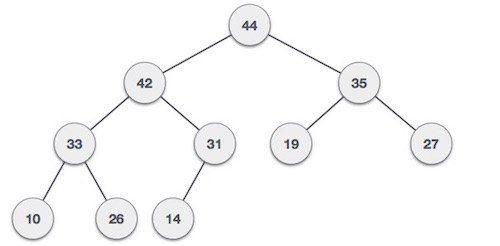
\includegraphics[scale=0.5]{figures/CM3/max_heap_example.jpg}
        \label{fig:my_label}
    \end{figure}
\end{frame}

\begin{frame}{Min Heap}
    Lorsque la valeur du nœud racine est inférieure ou égale à celle de l'un de ses enfants.
        \begin{exampleblock}{Entrée}
    \begin{center}
            \defin{35 33 42 10 14 19 27 44 26 31}
    \end{center}
    \end{exampleblock}
     \begin{figure}
        \centering
        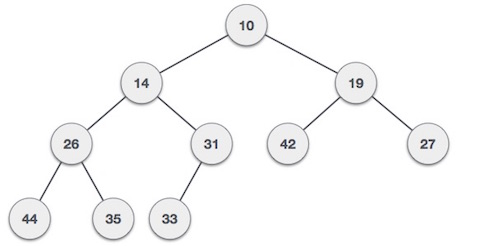
\includegraphics[scale=0.5]{figures/CM3/min_heap_example.jpg}
        \label{fig:my_label}
    \end{figure}
\end{frame}

\begin{frame}{Algorithme de construction d'un Max Heap}
    Nous allons utiliser le même exemple pour montrer comment créer un Max Heap. La procédure de création du tas min est similaire, mais nous choisissons des valeurs min au lieu de valeurs max.

Nous allons dériver un algorithme pour le Max Heap en insérant un élément à la fois. À tout moment, le tas doit conserver sa propriété.

\begin{alertblock}{Algorithme}
\begin{enumerate}
    \item Créer un nouveau nœud à la fin du tas.
    \item Attribuer une nouvelle valeur au noeud.
    \item Comparer la valeur de ce noeud enfant avec son parent.
    \item Si la valeur du parent est inférieure à celle de l'enfant, alors échangez-les.
    \item Répétez les étapes 3 et 4 jusqu'à ce que la propriété du tas soit respectée.
\end{enumerate}
\end{alertblock}
\end{frame}

\begin{frame}{Exemple de construction de Max Heap}
\foreach \n in {1,...,59}{
\only<\n>{
    \begin{figure}
        \centering
        \includegraphics[scale=0.65]{figures/CM3/max-heap-animation/frame_\n_delay-0.5s.jpg}
        \label{fig:my_label}
    \end{figure}
}
}
\end{frame}

\begin{frame}{Algorithme de suppression dans un Max Heap}
    Déterminons un algorithme de suppression dans le tas maximum. La suppression dans le tas Max (ou Min) se produit toujours à la racine pour supprimer la valeur maximale (ou minimale).

\begin{alertblock}{Algorithme}
\begin{itemize}
    \item Suppression du nœud racine.
    \item Déplacer le dernier élément du dernier niveau vers la racine.
    \item Comparer la valeur de ce noeud enfant avec son parent.
    \item Si la valeur du parent est inférieure à celle de l'enfant, échangez-les.
    \item Répétez les étapes 3 et 4 jusqu'à ce que la propriété "Heap" soit respectée.
\end{itemize}
\end{alertblock}
\end{frame}

\begin{frame}{Exemple de suppression dans un Max Heap}
    \foreach \n in {1,...,17}{
\only<\n>{
    \begin{figure}
        \centering
        \includegraphics[scale=0.65]{figures/CM3/max-heap-suppr/frame_\n_delay-0.7s.jpg}
        \label{fig:my_label}
    \end{figure}
}
}
\end{frame}

\section{Les graphes}

\begin{frame}{Un peu d'histoire}

L’histoire de la théorie des graphes débute avec les travaux d’Euler au \texttt{XVIII}e siècle.

\only<1>{
\begin{figure}
    \centering
    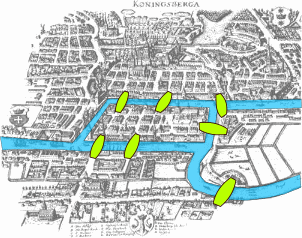
\includegraphics[scale=0.7]{figures/CM3/Konigsberg_bridges.png}
    \label{fig:my_label}
\end{figure}
}

\only<2>{
\begin{figure}
    \centering
    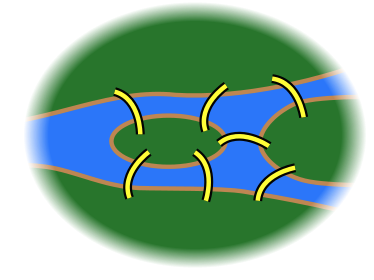
\includegraphics[scale=0.75]{figures/CM3/Konigsberg_bridges-1.png}
    \label{fig:my_label}
\end{figure}
}

\only<3>{
\begin{figure}
    \centering
    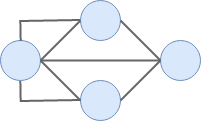
\includegraphics[scale=0.75]{figures/CM3/Konigsberg_bridges-2.png}
    \label{fig:my_label}
\end{figure}
}
\end{frame}

\begin{frame}{Définitions}
    \begin{exampleblock}{Graphe}
        un graphe est un couple G = (V, E) tel que :
    \begin{itemize}
        \item V un ensemble de sommets (aussi appelés \textit{nœuds} ou \textit{vertex});
        \item $E \subseteq \{\{x, y\} | (x, y) \in V^2 \wedge x \not\equal y\}$ un ensemble d'arêtes (aussi appelées \textit{liens}), qui sont des paires de sommets (c.-à-d. qu'une arête est associée à deux sommets distincts).
    \end{itemize}
    \end{exampleblock}
\end{frame}

\begin{frame}{Sommets et arêtes}
    \begin{exampleblock}{Sommets}
    \begin{itemize}
        \item Un élément simple;
        \item on le dessine habituellement par un point; 
        \item  \textbf{\defin{L'ensemble des sommets}} de G est noté $V(G)$ et on note $n = |V(G)|$
    \end{itemize}
    \end{exampleblock}
    
    \begin{exampleblock}{Arêtes}
    \begin{itemize}
        \item Un ensemble de deux éléments;
        \item On le dessine habituellement par une ligne entre les deux points;
        \item \textbf{\defin{L'ensemble des arêtes}} de G est noté $E(G)$ et on note $m = |V(G)|$
    \end{itemize}
    \end{exampleblock}
    
    \begin{exampleblock}{Le voisinage}
    Pour chaque sommet v, l'ensemble des noeuds qui sont connectés par une arête à ce noeud v est appelé le voisinage et est noté $N(v)$
    \end{exampleblock}
\end{frame}

\begin{frame}{Exemple de graphe}
    \begin{figure}
        \centering
        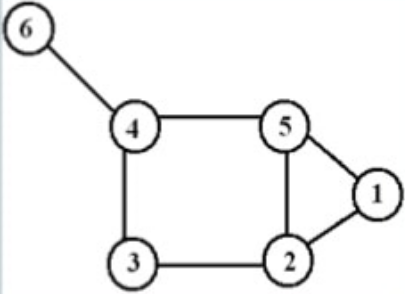
\includegraphics[scale=0.35]{figures/CM3/graph-example.png}
        \label{fig:my_label}
    \end{figure}
    \begin{itemize}
        \item n = 6 ; m = 7
        \item V(G) = \{1, 2, 3, 4, 5, 6\}
        \item E(G) = \{ (1,2), (1,5), (2,3), (2,5), (3,4), (4,5), (4,6) \}
        \item N(4) = \only<1>{\alert{?}} \only<2>{\alert{\{6, 5, 3\}}}
    \end{itemize}
\end{frame}


\begin{frame}{Graphe simple (non dirigé)}
    \begin{exampleblock}{Degré d'un sommet}
    On définit le degré d'un sommet $d(v)$ comme étant le nombre de voisins de V, on a donc :
    $d(v) = |N(v)|$
    \end{exampleblock}
    
    \begin{exampleblock}{Boucle (\textit{loop)}}
    Une boucle est une arête (v,v) , v étant un sommet.
    \end{exampleblock}
    
    \begin{exampleblock}{Définition d'un graphe simple}
    Un graphe simple est un graphe non dirigé sans \defin{boucle}.
    \end{exampleblock}
    
    \begin{alertblock}{Somme des degrés d'un graphe}
        Dans un graphe simple G, on a :
        \begin{equation*}
            \sum_{v_i \in V(G)}deg(v_i) = \only<1>{\alert{?}} \only<2>{\alert{2|E|}}
        \end{equation*}
    \end{alertblock}
    
\end{frame}

\begin{frame}{Graphe dirigé (\textit{digraph})}
    \begin{itemize}
        \item Les arêtes sont orientées;
        \item les boucles sont autorisées;
        \item les multi-arêtes sont autorisées.
    \end{itemize}
    
    \begin{figure}
        \centering
        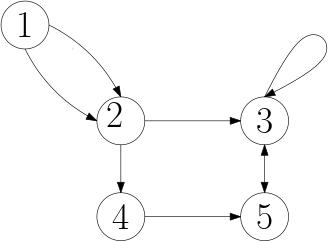
\includegraphics[scale=0.5]{figures/CM3/directed-graph.png}
        \label{fig:my_label}
    \end{figure}
\end{frame}

\begin{frame}{Les graphes pondérés}
    \begin{exampleblock}{Définition}
    Un graphe est dit \defin{pondéré} si chaque arête à un \defin{poids} associé.
    \end{exampleblock}
    
    \begin{figure}
        \centering
        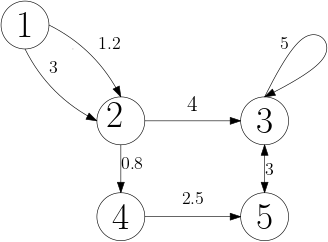
\includegraphics[scale=0.5]{figures/CM3/weighted-graph.png}
        \label{fig:my_label}
    \end{figure}
\end{frame}

\begin{frame}{Graphe biparti}
    \begin{exampleblock}{Définition}
    Un graphe est dit \defin{\textbf{biparti}} si l'ensemble des sommets $V$ peut être partitionné en deux ensembles $V_1$ et $V_2$ tel que $(u,v) \in E$ implique :
    \begin{itemize}
        \item soit $u \in V_1$ et $v \in V_2$
        \item soit $v \in V_1$ et $u \in V_2$
    \end{itemize}
    \end{exampleblock}

    \begin{figure}
        \centering
        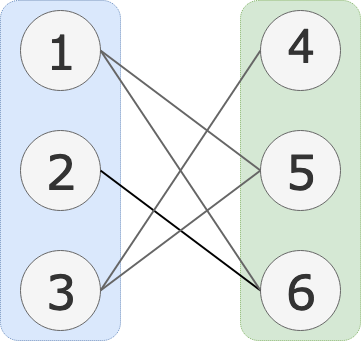
\includegraphics[scale=0.4]{figures/CM3/graph-bipartite.png}
        \label{fig:my_label}
    \end{figure}
\end{frame}

\begin{frame}{Quelques définitions}
    \begin{exampleblock}{Graphe connexe}
    Graphe dans lequel on peut relier, directement ou non, n'importe quel sommet à n'importe quel autre sommet du graphe par une chaîne d'arêtes.
\end{exampleblock}

\begin{figure}
    \centering
    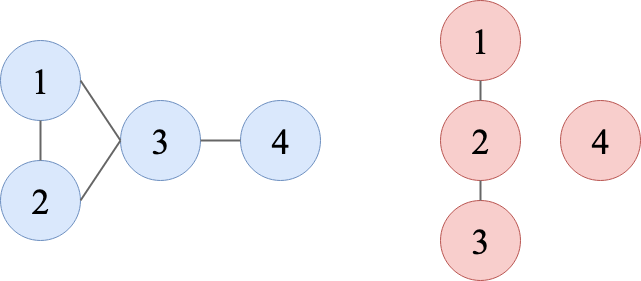
\includegraphics[scale=0.4]{figures/CM3/graph-connected.png}
    \label{fig:my_label}
\end{figure}
\end{frame}

\begin{frame}{Quelques définitions}
    \begin{exampleblock}{Chaîne}
        une \defin{\textbf{chaîne}} reliant x à y, notée $\mu$(x,y), est définie par une suite finie d'arêtes consécutives, reliant x à y. 
    \end{exampleblock}
    \begin{exampleblock}{Vocabulaire}
            \begin{itemize}
                \item Une \defin{\textbf{chaîne élémentaire}} est une chaîne ne passant pas deux fois par un même sommet, c'est-à-dire dont tous les sommets sont distincts;
                \item Une \defin{\textbf{chaîne simple}} est une chaîne ne passant pas deux fois par une même arête, c'est-à-dire dont toutes les arêtes sont distinctes.
            \end{itemize}
    \end{exampleblock}
    \begin{figure}
        \centering
        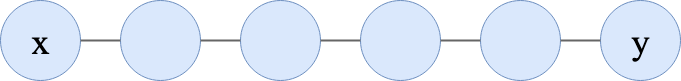
\includegraphics[scale=0.3]{figures/CM3/path.png}
        \label{fig:my_label}
    \end{figure}
\end{frame}


\begin{frame}{Quelques définitions}
    \begin{exampleblock}{Cycle}
Dans un graphe non orienté, un \defin{\textbf{cycle}} est une suite d'arêtes consécutives dont les deux sommets extrémités sont identiques.
\end{exampleblock}

\begin{figure}
    \centering
    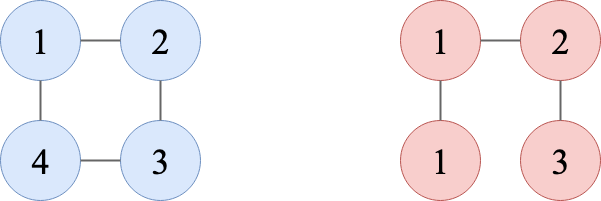
\includegraphics[scale=0.4]{figures/CM3/cycle-graph.png}
    \label{fig:my_label}
\end{figure}

\underline{Note:} Un \defin{\textbf{cycle}} est une \defin{chaîne simple} dont les deux extrémités sont identiques. 
\end{frame}



\begin{frame}{Les arbres}
    \begin{exampleblock}{Définition}
        Un graphe simple est un \defin{\textbf{arbre}} si il est \defin{connexe} et sans \defin{cycle}.
    \end{exampleblock}
    
    \begin{figure}
        \centering
        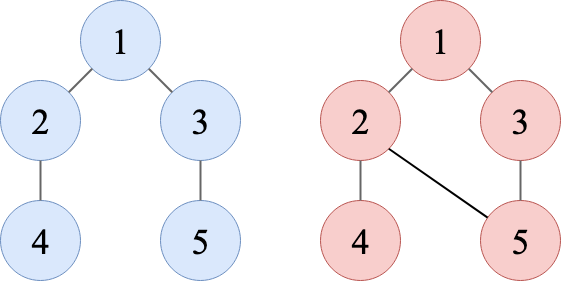
\includegraphics[scale=0.4]{figures/CM3/tree.png}
        \label{fig:my_label}
    \end{figure}
\end{frame}

\begin{frame}{Sous-graphe}
    \begin{exampleblock}{Définition}
        Un \defin{\textbf{sous-graphe}} G' d'un graphe G contient un sous-ensemble des sommets et des arêtes de G.
    \end{exampleblock}
    
    \begin{figure}
        \centering
        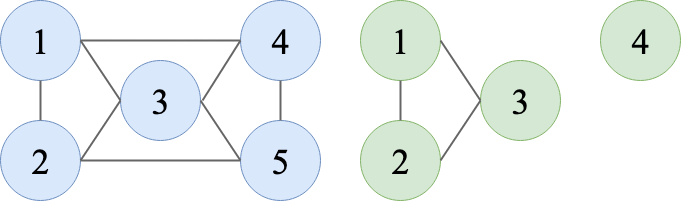
\includegraphics[scale=0.4]{figures/CM3/subgraph.png}
        \label{fig:my_label}
    \end{figure}
\end{frame}


\begin{frame}{Graphe planaire}
    \begin{exampleblock}{Définition}
            \begin{itemize}[<+->]
                \item Une \defin{\textbf{représentation}} d'un graphe G est une fonction qui associe chaque sommet $v \in V(G)$ ) un point $f(v)$ dans le plan et chaque  arête $u v$ à un courbe entre $f(u)$ et $f(v)$;
                \item Un point $f(e) \cap f(e')$ autre qu'un point commun est un \textbf{\defin{croisement}};
                \item Un graphe est \defin{\textbf{planaire}} si il a une \defin{représentation} sans \defin{croisement}
            \end{itemize}
    \end{exampleblock}
    \only<4>{
    \begin{figure}
        \centering
        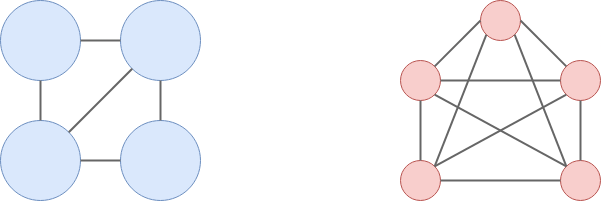
\includegraphics[scale=0.5]{figures/CM3/graph-planar.png}
        \label{fig:my_label}
    \end{figure}
    }
\end{frame}

\begin{frame}{Graphe complet}
    \begin{exampleblock}{Définition}
            Un graphe \textbf{\defin{complet}} est un graphe dont tous les sommets sont \defin{adjacents}. À \textit{isomorphisme} près, il n'existe qu'un seul graphe \defin{complet} non orienté d'ordre $n$, que l'on note $\mathcal{K}_n$.\\
            
            on appelle \defin{\textbf{clique}} un sous-ensemble de sommets induisant un sous-graphe complet de G.
    \end{exampleblock}
    
    \begin{figure}
        \centering
        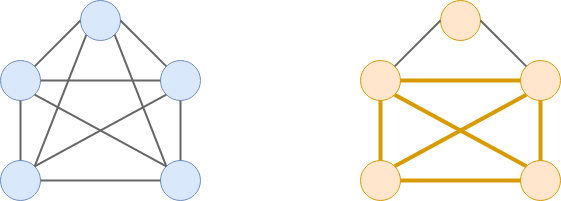
\includegraphics[scale=0.5]{figures/CM3/complete-graph.png}
        \label{fig:my_label}
    \end{figure}
\end{frame}

\begin{frame}{Graphe eulérien}
    \only<1>{
    \begin{exampleblock}{Définition}
    Un \defin{\textbf{ parcours eulérien}} d'un graphe non orienté est un chemin qui passe par toutes les arêtes, une fois par arête.
    Si un tel chemin revient au sommet de départ, on parle de \textbf{\defin{circuit eulérien}}.\\
    Un graphe qui admet un \defin{circuit eulérien} est dit \defin{eulérien}.
    \end{exampleblock}
    }
    \begin{alertblock}{Intuition}
    La notion de parcours \alert{eulérien} s'illustre avec le problème du \alert{\textbf{dessin de l'enveloppe}}. Il s'agit de tracer une enveloppe sans lever le crayon et sans dessiner plusieurs fois un même trait.\\
    Un parcours \alert{eulérien} correspond à un tracé d'un graphe sur une feuille sans lever le crayon.
    \end{alertblock}
    
    \only<2>{
    \begin{figure}
        \centering
        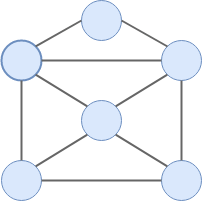
\includegraphics[scale=0.6]{figures/CM3/graph-euler.png}
        \label{fig:my_label}
    \end{figure}
    }
    
        \only<3>{
    \begin{figure}
        \centering
        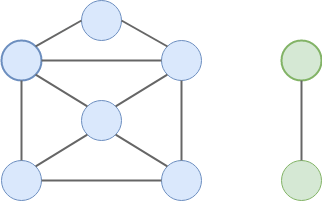
\includegraphics[scale=0.6]{figures/CM3/graph-euler-1.png}
        \label{fig:my_label}
    \end{figure}
    
    }
        \only<4>{
    \begin{figure}
        \centering
        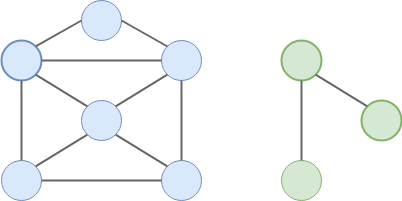
\includegraphics[scale=0.6]{figures/CM3/graph-euler-2.png}
        \label{fig:my_label}
    \end{figure}
    
    }
        \only<5>{
    \begin{figure}
        \centering
        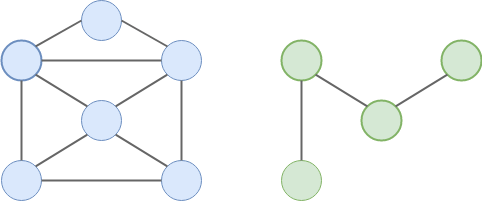
\includegraphics[scale=0.6]{figures/CM3/graph-euler-3.png}
        \label{fig:my_label}
    \end{figure}
    }
        \only<6>{
    \begin{figure}
        \centering
        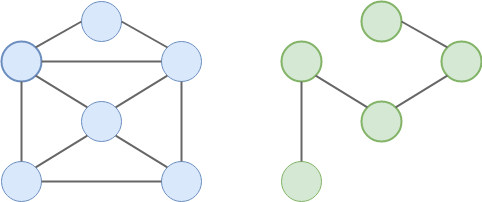
\includegraphics[scale=0.6]{figures/CM3/graph-euler-4.png}
        \label{fig:my_label}
    \end{figure}
    }
            \only<7>{
    \begin{figure}
        \centering
        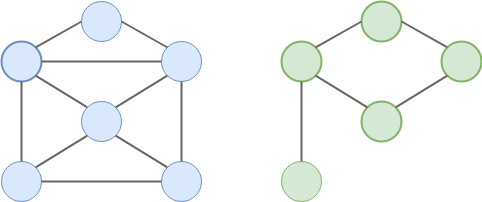
\includegraphics[scale=0.6]{figures/CM3/graph-euler-5.png}
        \label{fig:my_label}
    \end{figure}
    }
            \only<8>{
    \begin{figure}
        \centering
        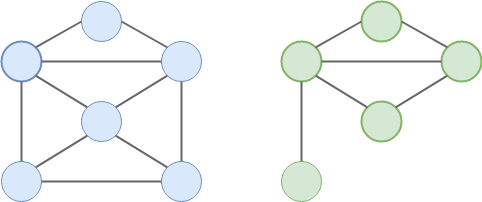
\includegraphics[scale=0.6]{figures/CM3/graph-euler-6.png}
        \label{fig:my_label}
    \end{figure}
    }
            \only<9>{
    \begin{figure}
        \centering
        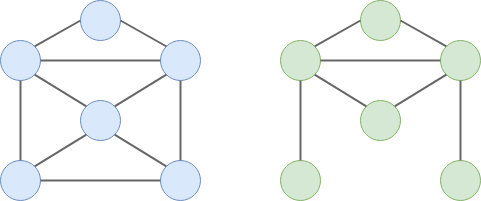
\includegraphics[scale=0.6]{figures/CM3/graph-euler-7.png}
        \label{fig:my_label}
    \end{figure}
    }
            \only<10>{
    \begin{figure}
        \centering
        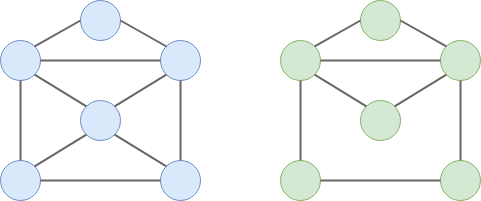
\includegraphics[scale=0.6]{figures/CM3/graph-euler-8.png}
        \label{fig:my_label}
    \end{figure}
    }
            \only<11>{
    \begin{figure}
        \centering
        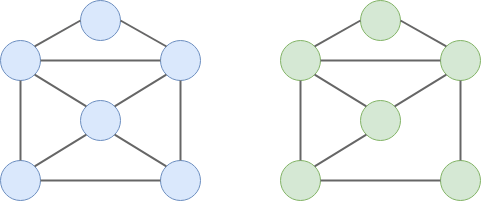
\includegraphics[scale=0.6]{figures/CM3/graph-euler-9.png}
        \label{fig:my_label}
    \end{figure}
    }
            \only<12>{
    \begin{figure}
        \centering
        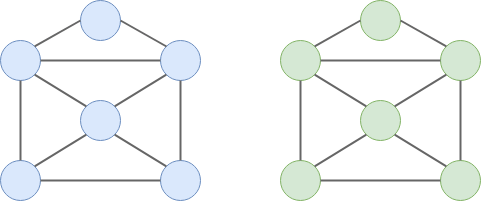
\includegraphics[scale=0.6]{figures/CM3/graph-euler-10.png}
        \label{fig:my_label}
    \end{figure}
    }
\end{frame}

\begin{frame}{Et notre histoire de ponts ?}
\only<1>{
\begin{figure}
    \centering
    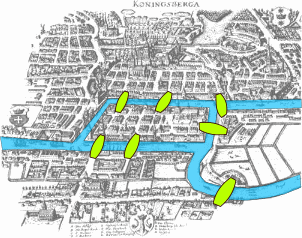
\includegraphics{figures/CM3/Konigsberg_bridges.png}
    \label{fig:my_label}
\end{figure}
}
\only<2>{
\begin{figure}
    \centering
    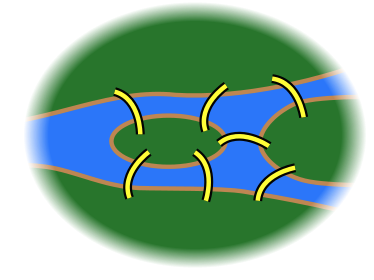
\includegraphics{figures/CM3/Konigsberg_bridges-1.png}
    \label{fig:my_label}
\end{figure}
}
\only<3>{

    \begin{figure}
        \centering
        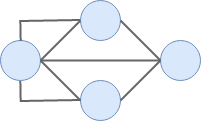
\includegraphics{figures/CM3/Konigsberg_bridges-2.png}
        \label{fig:my_label}
    \end{figure}
    \alert{\begin{center}
        Est-ce-que ce graphe est \alert{eulérien} ? \only<2>{Non \frownie{}}
    \end{center}}
    }
\end{frame}

\begin{frame}{Théorème d'Euler}
    \begin{exampleblock}{Théorème}
    Le théorème d'Euler se décline en deux caractérisations :
\begin{itemize}
    \item  Un graphe \defin{connexe} admet un \defin{\textbf{parcours eulérien}} si et seulement si ses sommets sont tous de degré \defin{pair} sauf au plus deux.
    \item  Un graphe \defin{connexe} admet un \textbf{circuit eulérien} si et seulement si tous ses sommets sont de degré \defin{pair}.
\end{itemize}
    \end{exampleblock}
    \only<2>{
    
    \begin{figure}
        \centering
        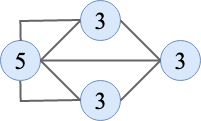
\includegraphics[scale=0.6]{figures/CM3/Konigsberg_bridges-3.png}
        \label{fig:my_label}
    \end{figure}
    }
\end{frame}

\begin{frame}{Graphe hamiltonien}
    \begin{exampleblock}{Définitions}
    \begin{itemize}
        \item Une \defin{\textbf{chaîne hamiltonienne}} est une chaîne qui passe une fois et une seule par chaque sommet du graphe.
        \item Un \defin{\textbf{cycle hamiltonien}} est une chaîne \defin{hamiltonienne} qui est cyclique.
    \end{itemize}
    \begin{alertblock}{Un peu d'histoire}
    Au $IX^e$ siècle, le poète indien \textit{Rudrata} a été le premier à trouver le problème des cycles/chemins \alert{hamiltoniens} sur un échiquier mais avec un cavalier. Il s'agit du \alert{problème du cavalier}. 
    \end{alertblock}
    \end{exampleblock}
\end{frame}

\begin{frame}{Graphe hamiltonien}
    \begin{exampleblock}{Définitions}
    \begin{itemize}
        \item Une \defin{\textbf{chaîne hamiltonienne}} est une chaîne qui passe une fois et une seule par chaque sommet du graphe.
        \item Un \defin{\textbf{cycle hamiltonien}} est une chaîne \defin{hamiltonienne} qui est cyclique.
    \end{itemize}
    \end{exampleblock}
    \begin{alertblock}{Quelques exemples}
    \only<1-2>{
    \begin{figure}
        \centering
        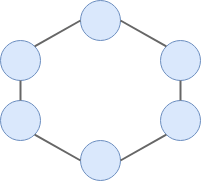
\includegraphics[scale=0.5]{figures/CM3/graph-hamiltonian.png}
        \label{fig:my_label}
    \end{figure}
    }
    \only<2>{
    \begin{center}
        \alert{\smiley{}}
    \end{center}
    }
    
    \only<3-4>{
    
    \begin{figure}
        \centering
        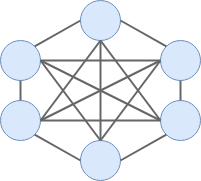
\includegraphics[scale=0.5]{figures/CM3/graph-hamiltonian-1.png}
        \label{fig:my_label}
    \end{figure}
    }
    \only<4>{
    \begin{center}
        \alert{\smiley{}}
    \end{center}
    }
    
    \only<5-6>{
    \begin{figure}
        \centering
        \includegraphics[scale=0.5]{figures/CM3/graph-hamiltonian-2.png}
        \label{fig:my_label}
    \end{figure}
    }
    \only<6>{
    \begin{center}
        \alert{\frownie{}}
    \end{center}
    }
    \end{alertblock}
\end{frame}

\begin{frame}{Caractérisation des graphes hamiltoniens}
\only<1>{
    \begin{center}
        \defin{Il n'existe pas de caractérisation pour les graphes hamiltoniens !}
    \end{center}
    }
    \only<2-3>{
    \begin{exampleblock}{Théorème de Dirac (1952)}
            Un graphe simple à n sommets ($n \geq 3$) dont chaque sommet est au moins de degré $\frac{n}{2}$ est \defin{hamiltonien}.
    \end{exampleblock}
    }
    
    \only<3-4>{
    \begin{exampleblock}{Théorème de Ore (1960)}
            Un graphe simple à n sommets ($n \geq 3$) tel que la somme des degrés de toute parie de sommets non adjacents vaut au moins $n$ est hamiltonien.
    \end{exampleblock}
    \only<3>{
    \begin{center}
        Le théorème de \textit{Dirac} est un cas particulier du théorème de \textit{Ore} : en effet, si chaque sommet est de degré au moins $\frac{n}{2}$ , alors la somme des degrés de n'importe quelle paire de sommets, adjacents ou pas, est au moins n. 
    \end{center}
    }
    }
    
    \only<4>{
    \begin{exampleblock}{Théorème de Pósa (1962)}
        Un graphe simple à $n$ sommets ($n\geq 3$) tel que :
        \begin{enumerate}
            \item pour tout entier $k$ tel que $ 1\leq k<\frac {n-1}{2}$ le nombre de sommets de degré inférieur ou égal à $k$ est inférieur à $k$
            \item le nombre de sommets de degré inférieur ou égal à $\frac{n - 1}{2}$ est inférieur ou égal à $\frac{n - 1}{2}$
        \end{enumerate}
    est hamiltonien.
    \end{exampleblock}
    \begin{center}
        On remarque que la condition 2 est comprise dans la condition 1 quand $n$ est pair, et n'a donc d'intérêt que lorsque $n$ est impair. 
    \end{center}
    }
\end{frame}

\begin{frame}{Prenons un exemple}
    \begin{exampleblock}{Exemple}
        Le graphe ci-contre possède 6 sommets. Il est \defin{hamiltonien} : les sommets ont été ordonnés de manière à mettre en évidence un \defin{cycle hamiltonien}, c'est le cycle extérieur rouge. 
    \end{exampleblock}
    \begin{figure}
        \centering
        \includegraphics[scale=0.6]{figures/CM3/graph-theorem-hamiltonian.png}
        \label{fig:my_label}
    \end{figure}
\end{frame}

\begin{frame}{Prenons un exemple}
        \begin{exampleblock}{Théorème de Dirac (1952)}
            Un graphe simple à n sommets ($n \geq 3$) dont chaque sommet est au moins de degré $\frac{n}{2}$ est \defin{hamiltonien}.
    \end{exampleblock}
    
        \begin{figure}
        \centering
        \includegraphics[scale=0.55]{figures/CM3/graph-theorem-hamiltonian.png}
        \label{fig:my_label}
    \end{figure}
    Le théorème de \textit{Dirac} ne permet pas de prouver qu'il est \defin{hamiltonien}. Pour cela, tous les sommets devraient au moins être de degré 3 , or il y a un sommet de degré 2.
\end{frame}

\begin{frame}{Prenons un exemple}
    \begin{exampleblock}{Théorème de Ore (1960)}
            Un graphe simple à n sommets ($n \geq 3$) tel que la somme des degrés de toute parie de sommets non adjacents vaut au moins $n$ est hamiltonien.
    \end{exampleblock}
    
        \begin{figure}
        \centering
        \includegraphics[scale=0.55]{figures/CM3/graph-theorem-hamiltonian.png}
        \label{fig:my_label}
    \end{figure}
Le théorème de \textit{Ore} n'est pas plus utile, car les sommets non adjacents a et b vérifient deg(a) + deg(b) = 3 + 2 = 5, or on devrait avoir au moins 6.
\end{frame}

\begin{frame}{Prenons un exemple}
    \begin{exampleblock}{Théorème de Pósa (1962)}
        \begin{enumerate}
            \item pour tout entier $k$ tel que $ 1\leq k<\frac {n-1}{2}$ le nombre de sommets de degré inférieur ou égal à $k$ est inférieur à $k$
            \item le nombre de sommets de degré inférieur ou égal à $\frac{n - 1}{2}$ est inférieur ou égal à $\frac{n - 1}{2}$
        \end{enumerate}
    \end{exampleblock}
     \begin{figure}
        \centering
        \includegraphics[scale=0.35]{figures/CM3/graph-theorem-hamiltonian.png}
        \label{fig:my_label}
    \end{figure}
    En revanche, le théorème de \textit{Pósa} permet de déterminer que le graphe est \defin{hamiltonien}, car il y a 0 sommet de degré 1 et 1 sommet de degré 2: la condition 1 est remplie (0 < 1 et 0 + 1 < 2 ).
\end{frame}
\section{Algorithme de Dijkstra}

\begin{frame}{Problème du plus court chemin}
    \begin{exampleblock}{Énoncé du problème}
    Étant donné un graphe non-orienté, dont les arêtes sont munies de poids, et deux sommets de ce graphe, trouver un chemin entre les deux sommets dans le graphe, de poids minimum.
    \end{exampleblock}
    \begin{alertblock}{Principe de l'algorithme}
    \begin{enumerate}
        \item On choisit le sommet accessible de distance minimale comme sommet à explorer;
        \item A partir de ce sommet, on explore ses voisins et on met à jour les distances pour chacun. On ne met à jour la distance que si elle est inférieure à celle que l’on avait auparavant;
        \item On répète jusqu’à ce que l’on arrive au point d’arrivée ou jusqu’à ce que tous les sommets aient été explorés.
    \end{enumerate}
    \end{alertblock}
\end{frame}

\begin{frame}{Prenons un exemple}
\only<1>{
    \begin{exampleblock}{Énoncé de l'exemple}
    L'exemple ci-contre montre les étapes successives dans la résolution du chemin le plus court dans un graphe. Les nœuds symbolisent des villes identifiées par une lettre et les arêtes indiquent la distance entre ces villes. On cherche à déterminer le plus court trajet pour aller de la ville A à la ville J. 
    \end{exampleblock}
        \begin{figure}
        \centering
        \includegraphics[scale=0.20]{figures/CM3/Djikstra-1.png}
        \label{fig:my_label}
    \end{figure}
    }
    \only<2>{
    \underline{Étape 1:} on choisit la ville A. On met à jour les villes voisines de A qui sont B, C, et E. Leurs distances deviennent respectivement 85, 217, 173, tandis que les autres villes restent à une distance infinie.
    \begin{figure}
        \centering
        \includegraphics[scale=0.30]{figures/CM3/Djikstra-2.png}
        \label{fig:my_label}
    \end{figure}
    }
    \only<3>{
    \underline{Étape 2:} on choisit la ville B. En effet, c'est la ville hors du sous-graphe qui est à la distance minimale (85). On met à jour le seul voisin (F). Sa distance devient 85+80 = 165.
    \begin{figure}
        \centering
        \includegraphics[scale=0.30]{figures/CM3/Djikstra-3.png}
        \label{fig:my_label}
    \end{figure}
    }
    \only<4>{
    \underline{Étape 3:} on choisit F. On met à jour le voisin I (415).
        \begin{figure}
        \centering
        \includegraphics[scale=0.30]{figures/CM3/Djikstra-4.png}
        \label{fig:my_label}
    \end{figure}
    }
    
    \only<5>{
    \underline{Étape 4 :} on choisit E. On met à jour le voisin J (675).
            \begin{figure}
        \centering
        \includegraphics[scale=0.30]{figures/CM3/Djikstra-5.png}
        \label{fig:my_label}
    \end{figure}
    }
    
    \only<6>{
    \underline{Étape 5 :} la distance la plus courte en dehors du sous-graphe est maintenant celle de la ville C. On choisit donc C. On met à jour la ville G (403) et la ville H (320).
              \begin{figure}
        \centering
        \includegraphics[scale=0.30]{figures/CM3/Djikstra-6.png}
        \label{fig:my_label}
    \end{figure}
    }
    \only<7>{
    \underline{Étape 6 :} la distance la plus courte en dehors du sous-graphe est maintenant celle de la ville H (320). On choisit donc H. On met à jour la ville D (503) et la ville J (487< 675).
    \begin{figure}
        \centering
        \includegraphics[scale=0.30]{figures/CM3/Djikstra-7.png}
        \label{fig:my_label}
    \end{figure}
    }
    \only<8>{
    \underline{Étape 7 :} la distance la plus courte suivante est celle de la ville G. On choisit G. La mise à jour ne change aucune autre distance.
    \begin{figure}
        \centering
        \includegraphics[scale=0.30]{figures/CM3/Djikstra-8.png}
        \label{fig:my_label}
    \end{figure}
    }
    
    \only<9>{
    \underline{Étape 8 :} la distance la plus courte suivante est celle de la ville I. La distance de la ville voisine J n'est pas modifiée car la distance existante est inférieure à celle que l'on obtiendrait en passant par I (415 + 84 > 487).
    \begin{figure}
        \centering
        \includegraphics[scale=0.30]{figures/CM3/Djikstra-9.png}
        \label{fig:my_label}
    \end{figure}
    }
    
    \only<10>{
    \underline{Étape 9 :} la ville dont la distance est la plus courte est J (487). On choisit J et on l'ajoute au sous-graphe. On s'arrête puisque la ville d'arrivée est maintenant dans le sous-graphe.
    \begin{figure}
        \centering
        \includegraphics[scale=0.30]{figures/CM3/Djikstra-10.png}
        \label{fig:my_label}
    \end{figure}
    }
    \only<11>{
    En neuf étapes, on peut déterminer le chemin le plus court menant de A à J, il passe par C et H et mesure 487 km. 
        \begin{figure}
        \centering
        \includegraphics[scale=0.30]{figures/CM3/Djikstra-11.png}
        \label{fig:my_label}
    \end{figure}
    
    }
\end{frame}



\section{Coloration de graphes}
\begin{frame}{Nombre chromatique}
    \begin{exampleblock}{Définition}
            \begin{itemize}
                \item Une \defin{\textbf{k-coloration}} d'un graphe $G$ est un étiquetage $f$ : $V(G) \rightarrow \{ 1, 2, \ldots, k \}$;
                \item Les étiquettes sont des \defin{couleurs};
                \item Les sommets avec une couleur $i$ sont une \defin{classe de couleurs};
                \item Une \defin{k-coloration} $f$ est \textbf{\defin{propre}} si $f(x) \not\equal f(y)$ quand $x$ et $y$ sont adjacents;
                \item Le \defin{\textbf{nombre chromatique}} $\chi(G)$ est le minimum $k$ tel
                que G a une \defin{k-coloration propre};
                \item On note $\omega(G)$ le \defin{\textbf{nombre de clique}} la taille de la plus grande \defin{clique} d'un graphe;
                \item On note $\alpha(G)$ la taille du plus grand \textbf{\defin{ensemble indépendant}}, c'est-à-dire un ensemble de sommets deux à deux non \defin{adjacent}.
            \end{itemize} 
    \end{exampleblock}
\end{frame}

\begin{frame}{Exemple sur le nombre chromatique}
    \begin{exampleblock}{Rappel}
        Une \defin{k-coloration} $f$ est \textbf{\defin{propre}} si $f(x) \not\equal f(y)$ quand $x$ et $y$ sont adjacents;    
    \end{exampleblock}
    \only<1>{
        \begin{figure}
        \centering
        \includegraphics[scale=0.5]{figures/CM3/graph-planar.png}
        \label{fig:my_label}
    \end{figure}
    \alert{\begin{center}
        Quel est le nombre chromatique ?
    \end{center}}
    }
    \only<2>{
    \begin{figure}
        \centering
        \includegraphics[scale=0.5]{figures/CM3/chromatic-1.png}
        \label{fig:my_label}
    \end{figure}
    }
    
    \only<3>{
    \begin{figure}
        \centering
        \includegraphics[scale=0.5]{figures/CM3/chromatic-2.png}
        \label{fig:my_label}
    \end{figure}
    }
\end{frame}

\begin{frame}{Exemple sur le nombre de clique}
    \begin{exampleblock}{Rappel}
        On note $\omega(G)$ le \defin{\textbf{nombre de clique}} la taille de la plus grande \defin{clique} d'un graphe
    \end{exampleblock}
    
    \only<1>{
    \begin{figure}
        \centering
        \includegraphics[scale=0.5]{figures/CM3/graph-clique-1.png}
        \label{fig:my_label}
    \end{figure}
    }
    
    \only<2>{
    \begin{figure}
        \centering
        \includegraphics[scale=0.5]{figures/CM3/graph-clique-2.png}
        \label{fig:my_label}
    \end{figure}
    }
    \only<3>{
    \begin{figure}
        \centering
        \includegraphics[scale=0.5]{figures/CM3/graph-clique-3.png}
        \label{fig:my_label}
    \end{figure}
    }
\end{frame}

\begin{frame}{Exemple sur les ensembles indépendant}
    \begin{exampleblock}{Rappel}
      On note $\alpha(G)$ la taille du plus grand \textbf{\defin{ensemble indépendant}}, c'est-à-dire un ensemble de sommets deux à deux non \defin{adjacent}.
    \end{exampleblock}
    
    \only<1>{
    
    \begin{figure}
        \centering
        \includegraphics[scale=0.5]{figures/CM3/graph-stable-1.png}
        \label{fig:my_label}
    \end{figure}
    }
    \only<2>{
    
    \begin{figure}
        \centering
        \includegraphics[scale=0.5]{figures/CM3/graph-stable-2.png}
        \label{fig:my_label}
    \end{figure}
    }
    \only<3>{
    
    \begin{figure}
        \centering
        \includegraphics[scale=0.5]{figures/CM3/graph-stable-3.png}
        \label{fig:my_label}
    \end{figure}
    }
    \only<4>{
    
    \begin{figure}
        \centering
        \includegraphics[scale=0.5]{figures/CM3/graph-stable-4.png}
        \label{fig:my_label}
    \end{figure}
    }
    \only<5>{
    
    \begin{figure}
        \centering
        \includegraphics[scale=0.5]{figures/CM3/graph-stable-5.png}
        \label{fig:my_label}
    \end{figure}
    }
\end{frame}

\begin{frame}{Théorèmes sur la coloration}
    \begin{exampleblock}{Théorème 1}
        Soit G un graphe à n sommets, on a la relation suivante:
        \begin{equation*}
            \frac{n}{\alpha} \leq \chi
        \end{equation*}
        
        \begin{proof}
            Supposons que G est colorié avec $\chi$ couleurs. Comme chaque \defin{classe de couleurs} est indépendant, la taille de chaque classe de couleur est au plus $\alpha$. Soient les classes de couleur $V_1, V_2, \ldots,  V_\alpha$. On obtient:
            
            \begin{equation*}
                n = \sum_{i=1}^\chi |V_i| \leq \chi \alpha 
            \end{equation*}
        \end{proof}
    \end{exampleblock}
\end{frame}

\begin{frame}{Théorèmes sur la coloration}
    \begin{exampleblock}{Théorème 2}
        Soit $\Delta$ le degré maximal dans un graphe, on a la relation suivante:
        \begin{equation*}
            \chi \leq \Delta + 1
        \end{equation*}
\only<1>{        
        \begin{proof}
  Colorez le premier sommet avec la première couleur et faire pour les n-1 sommets restants:
    \begin{itemize}
        \item On prend un sommet et on le colore avec la couleur la plus basse
    qui n'a pas été utilisée sur les sommets précédemment colorés
    qui lui sont adjacents;
        \item Si toutes les couleurs précédemment utilisées apparaissent sur les sommets adjacents à v, attribuez-lui une nouvelle couleur.
    \end{itemize}
        \end{proof}
}
    \end{exampleblock}
\only<2>{    
    \begin{figure}
        \centering
        \includegraphics[scale=0.5]{figures/CM3/color-greedy.png}
        \label{fig:my_label}
    \end{figure}
    \begin{center}
        \alert{Quelle est la valeur de $\Delta$ ?}
    \end{center}
}

\only<3>{    
    \begin{figure}
        \centering
        \includegraphics[scale=0.5]{figures/CM3/color-greedy-1.png}
        \label{fig:my_label}
    \end{figure}
}

\only<4>{    
    \begin{figure}
        \centering
        \includegraphics[scale=0.5]{figures/CM3/color-greedy-2.png}
        \label{fig:my_label}
    \end{figure}
}

\only<5>{    
    \begin{figure}
        \centering
        \includegraphics[scale=0.5]{figures/CM3/color-greedy-3.png}
        \label{fig:my_label}
    \end{figure}
}

\only<6>{    
    \begin{figure}
        \centering
        \includegraphics[scale=0.5]{figures/CM3/color-greedy-4.png}
        \label{fig:my_label}
    \end{figure}
}

\only<7>{    
    \begin{figure}
        \centering
        \includegraphics[scale=0.5]{figures/CM3/color-greedy-5.png}
        \label{fig:my_label}
    \end{figure}
}

\only<8>{    
    \begin{figure}
        \centering
        \includegraphics[scale=0.5]{figures/CM3/color-greedy-6.png}
        \label{fig:my_label}
    \end{figure}
}

\only<9>{    
    \begin{figure}
        \centering
        \includegraphics[scale=0.5]{figures/CM3/color-greedy-7.png}
        \label{fig:my_label}
    \end{figure}
}

\end{frame}



\section{Représentation des graphes}
\begin{frame}{Matrice d'adjacence}
    \begin{exampleblock}{Définition}
    Supposons que $G=(V,E)$ est un graphe simple, où |V| = n. Supposons aussi que les sommets de G sont numérotés arbitrairement $v_{1},\ldots ,v_{n}$ . La matrice d’adjacence A de G se rapportant à cet ensemble de sommets est la matrice n × n \textit{booléenne} A avec:
\begin{equation*}
  a_{ij} =
    \begin{cases}
      1 & \text{si} (v_i,v_j) \in E\\
      0 & \text{sinon.}
    \end{cases}       
\end{equation*}
    \end{exampleblock}
\end{frame}

\begin{frame}{Exemple de matrice d'adjacence}
    \begin{minipage}{0.6\textwidth}
    \begin{figure}
        \centering
        \includegraphics[scale=0.3]{figures/CM3/adj-matrix.png}
        \label{fig:my_label}
    \end{figure}
    \end{minipage}
    \begin{minipage}{0.35\textwidth}
    $$
    \begin{pmatrix}
\quad & \boldsymbol{v_1} & \boldsymbol{v_2} & \boldsymbol{v_3} & \boldsymbol{v_4} & \boldsymbol{v_5} & \boldsymbol{v_6}\\
\boldsymbol{v_1} & 1 & 1 & 0 & 0 & 1 & 0\\
\boldsymbol{v_2} & 1 & 0 & 1 & 0 & 1 & 0\\
\boldsymbol{v_3} & 0 & 1 & 0 & 1 & 0 & 0\\
\boldsymbol{v_4} & 0 & 0 & 1 & 0 & 1 & 1\\
\boldsymbol{v_5} & 1 & 1 & 0 & 1 & 0 & 0\\
\boldsymbol{v_6} & 0 & 0 & 0 & 1 & 0 & 0
\end{pmatrix}
$$
    \end{minipage}
\end{frame}

\begin{frame}{Liste d'arêtes}
    \begin{exampleblock}{Liste d'arêtes}
        \begin{minipage}{0.6\textwidth}
    \begin{figure}
        \centering
        \includegraphics[scale=0.3]{figures/CM3/adj-matrix.png}
        \label{fig:my_label}
    \end{figure}
    \end{minipage}
    \begin{minipage}{0.35\textwidth}
    \begin{description}
        \item 1 1
        \item 1 2
        \item 1 5
        \item 2 3
        \item 2 5
        \item 3 4
        \item 4 5
        \item 4 6
    \end{description}
    \end{minipage}
    \end{exampleblock}
\end{frame}


\begin{frame}{Liste d'adjacence}
        \begin{exampleblock}{Liste d'adjacence}
        \begin{minipage}{0.6\textwidth}
    \begin{figure}
        \centering
        \includegraphics[scale=0.3]{figures/CM3/adj-matrix.png}
        \label{fig:my_label}
    \end{figure}
    \end{minipage}
    \begin{minipage}{0.35\textwidth}
    \begin{description}
        \item 1 1 2 5
        \item 2 3 5
        \item 3 2 4
        \item 4 3 5
        \item 5 1 2 4
        \item 6 4
    \end{description}
    \end{minipage}
    \end{exampleblock}
\end{frame}

\begin{frame}{Liste d'arêtes pour les graphes pondérés}
\begin{exampleblock}{Liste d'arêtes pour les graphes pondérés}
        \begin{minipage}{0.6\textwidth}
    \begin{figure}
        \centering
        \includegraphics[scale=0.3]{figures/CM3/weighted-graph.png}
        \label{fig:my_label}
    \end{figure}
    \end{minipage}
    \begin{minipage}{0.35\textwidth}
    \begin{description}
        \item 1 2 1.2
        \item 1 2 3
        \item 2 3 4
        \item 2 4 0.8
        \item 3 3 5
        \item 3 5 3
        \item 4 5 2.5
        \item 5 3 3
    \end{description}
    \end{minipage}
    \end{exampleblock}
\end{frame}

\end{document}